% Karrera Amarierako Proiektua egiteko LaTeX txantiloia
% itsas.ehu.es/workgroups/latex
% Unai Martinez Corral
% umartinez012@ikasle.ehu.es
%
% <- att_main.tex

Txantiloiaren erabilera zuzena da, hau da, dauden fitxategietan edukia beste edozein \LaTeX{} dokumentutan egin bezala idaztearekin nahikoa dugu. Erabilitako paketeek ezarri litzaketen mugak izan behar ditugu kontuan, eta berriren bat kargatzekotan ordenari erreparatu behar diogu.

Bete beharreko baldintza bakarra dago: goiburuetan azpiatalak ondo adierazi daitezen \emph{titlesubsection} erabili behar da \emph{subsection} ordez\footnote{\emph{GNU/Linux}en \emph{grep} erabilita zuzenean egin dezagu bihurketa.}.

Kodea garbi mantendu eta itxurari dagozkionak ahal den heinean banaturik mantentzeko hainbat fitxategi daude \emph{config} karpetan eta \emph{main.tex} fitxategian zenbait komando berri agertzen dira. Jarraian hauek azalduko dira, kapitulu zein atalak moldatu, gehitu zein kentzeko prozedura adierazteko.

\subsection*{main.tex}\addcontentsline{toc}{subsection}{main.tex}

\begin{verbatim}
\documentclass[a4paper,titlepage,10pt,oneside]{report}
\end{verbatim}

\emph{report} klasea dugu oinarri, alde bakarrekoa, DIN A4 formatuarekin. \emph{article} erabili nahi izatekotan, \emph{minitoc} paketeari dagozkion \emph{(do)minitoc}, \emph{(do)minilof} eta \emph{(do)minilot} aginduen kudeaketa aldatu beharko litzateke (ikus \emph{config.tex} eta \emph{config\_index.tex}), paketearen dokumentazioan adierazitakoen arabera. Pakete hori erabiltzen ez bada, aldaketa zuzena da.

Orriaren tamainari dagokionez, aldatzekotan kapitulu eta atalen orrietan distantziak berrikusi beharko lirateke (ikus \emph{config\_titles.tex}). Letraren tamaina aldatzean ere baliteke aldaketa txikiak somatzea.

\begin{verbatim}
\usepackage{import}
\inputfrom{./config/}{config.tex}
\end{verbatim}

Azpikarpetatan dauden fitxategiak kargatu eta hauetan kokapen erlatiboak erabili ahal izateko \emph{import} paketea kargatu da lehenik, eta honekin \emph{config} karpeta barruko konfigurazio fitxategi nagusia.

\begin{verbatim}
\begin{document}
\end{verbatim}

\begin{verbatim}
\DOpresetDOtitlepg
\end{verbatim}

Dokumentua hasi eta berehala \emph{config.tex} fitxategian definituta dagoen \emph{DOpresetDOtitlepg} komandoak euskaraz aurkezpena zuzenena izan dadin beharreko komandoak exekutatzen ditu, zenbakitzearen eta gaien aurkibidearen sakontasuna ezartzen ditu, kapituluen zenbakitzea zeroan abiarazten du, \emph{minitoc}ek eskatutakoak exekutatzen ditu, portada aurkezten du eta orrialde berri batean hasteko prestatzen du dokumentua.

\begin{verbatim}
\chapter{Aurkibide orokorra} \DOtls
\end{verbatim}

Lehenengo kapitulua, zerogarrena, \emph{Aurkibide orokorra} dugu. \emph{config\_index.tex} fitxategian definitutako \emph{DOtls} komandoak orrien zenbakitzea erromatarrera aldatu eta \emph{tableofcontents}, \emph{listoffigures} eta \emph{listoftables} exekutatzen ditu. Sekzio bezala gehitzen ditu aurkibidera, eta baten batek orri bat baino gehiago izatekotan goiburuak bat etor daitezen ezartzen ditu. Azkenik, berriz ere aldatzen du orrien zenbakitzea arabiarrera eta 1 balioa esleitzen dio.

\begin{verbatim}
\chapter{Memoria}
\pagestyle{empty}%Anie - ohkis.sourceforge.net
%Unai Martinez Corral
%umartinez012@ikasle.ehu.es
%
% <- anie.tex

\vspace*{.30\textheight}
\begin{flushright}
\begin{minipage}{0.65\textwidth}
\begin{flushright}
\itshape
``...hor egongo da begira.\\

\vspace{1.5ex}
Tú no nos diste el euskera,\\
pero nos diste la vida.\\
Nos llevaste a la ikastola,\\
aprendimos enseguida.\\
Ya es hora de que entiendas\\
el canto que nos motiva.\\
Esta txapela es tuya,\\
ay nire amatxu querida.''

\bigskip

\normalfont
\small{Xabier Paya}\\
\scriptsize{2006ko Bizkaiko Bertsolari Txapelketa}
\end{flushright}
\end{minipage}
\end{flushright}
\clearpage\pagestyle{body}
\DOmtls{\DOmtoc\DOmlof\DOmlot\DOmlos}
\end{verbatim}

Memoriaren hasiera adierazi eta berehala, goiburu eta oinik ez dituen estiloa ezartzen da eskaintza aurkezteko, \emph{config\_hdr.tex} fitxategian definitutako eta orokorrean erabiliko den \emph{body} estilora bueltatu baino lehen.

\emph{DOmtls} komandoak, \emph{DOtls}ek egin antzera zenbakitzea eta goiburuak moldatuz, kapituluko gaien aurkibidea (\emph{DOmtoc}), irudien zerrenda (\emph{DOmlof}), taulen zerrenda (\emph{DOmlot}) edota ikurren zerrenda (\emph{DOmlos}) aurkezten ditu. Lehenengo hirurak sortzeko \emph{minitoc} paketeak eskainitakoak erabiltzen diren bitartean, ikurren zerrendak zuzenean \emph{symbols.tex} fitxategiko edukia kargatzen du.

\begin{verbatim}
%Anie - ohkis.sourceforge.net
%Unai Martinez Corral
%umartinez012@ikasle.ehu.es
%
% <- anie.tex

\section{Sarrera}

2007 urtean zehar \emph{Iñaki Silanes}ek, \textbf{U}niversidad del \textbf{P}aís \textbf{V}asco \textbf{/} \textbf{E}uskal \textbf{H}erriko \textbf{U}nibertsitateko\footnote{\url{www.ehu.es}} \textbf{ITSAS}\footnote{\url{itsas.ehu.es}} Software Libre Taldeko kideak, \LaTeX{}\footnote{\url{en.wikipedia.org/wiki/LaTeX}} eta \emph{OpenDocument}\footnote{\url{en.wikipedia.org/wiki/OpenDocument}} formatuetan Unibertsitatean gazteleraz, euskaraz zein ingelesez Karrera Amaierako Proiektuak zein Doktorego Tesiak aurkezteko txantiloiak eskaintzeko helburuarekin \emph{Plantillas para Proyecto de Fin de Carrera} lan taldea\footnote{\url{itsas.ehu.es/workgroups/plantillas_proyecto_fin_de_carrera}} osatu zuen.

2010 urtean \emph{Digna González} eta \emph{Unai Martinez}ek lan talde berrian\footnote{\url{itsas.ehu.es/workgroups/latex}} \emph{Iñaki Silanes}en lana \emph{\LaTeX{}} erabiltzeko hainbat argibide, erreferentzia, aurkezpen eta abarrekin bateratu zuten eta material bera baliatuz zenbait ikastaro eman.

Idazleak, \textbf{Bi}lboko \textbf{I}ndustria \textbf{I}ngeniaritza \textbf{T}eknikoko \textbf{U}nibertsitate \textbf{E}skolan\footnote{\url{www.industria-ingeniaritza-tekniko-bilbao.ehu.es}} Karrera Amaierako Proiektua euskaraz idazteko orduan eskuragarri zeuden txantiloiek premia\footnote{\url{www.industria-ingeniaritza-tekniko-bilbao.ehu.es/p229-content/eu/contenidos/normativa/euiti_bi_pfc/eu_nor_gral/normativa_gral_fin_carrera.html}} guztiak asetzen ez zituztenez, aipatutako lan taldeetan bildutakoak oinarri, eskuartean duzun txantiloi berria egin du. \hyperref[tab:comp]{\ref*{tab:comp} taula}k \emph{Iñaki Silanes}ek eskainitakoekiko ezberdintasun nagusiak biltzen ditu.

\begin{table}[!htp]
\begin{tabular}{c c c c l}
& \bfseries Hizkuntza & \bfseries Formatua & \bfseries Klasea & \\
&&&&\\
\multirow{2}{*}{\bfseries Iñaki Silanes} & EU & \LaTeX{} & \multirow{2}{*}{\emph{itsas\_pfc.cls}} & \multirow{2}{*}{\emph{book} oinarri}\\
& ES EN & OpenDocument & & \\
&&&&\\
\bfseries Unai Martinez & EU & \LaTeX{} & \emph{report} & \emph{config} fitxategietan moldatuta\\
\end{tabular}
\caption{\emph{Iñaki Silanes}en txantiloiekin konparaketa.}
\label{tab:comp}
\end{table}

Horietaz gain, hurrengo berrikuntzak ditu honek:

\begin{itemize}
\item{Kapitulu, atal, azpiatal, azpiazpiatal, irudi eta taulak zenbakitu eta izendatzean zenbakia azaltzen da lehenengo, puntu ordinala ondoren eta hitza azkenik.}
\item{\emph{babel}ek \emph{basque} aukeratzean ezatzen duen data komandoaren ordez \emph{gaur} sortu da.}
\item{\emph{Kapitulu}en izen gisa \emph{Dokumentu} ezarri da.}
\item{BI-IITUEko web gunean soilik DOC formatuan eskuragarri dauden txantiloiak erabili dira \emph{Kapitulu/Dokumentu}en portadak diseinatzeko.}
\item{Atalen goiburuak aldatu dira.}
\item{Ikurren Zerrenda gehitu da.}
\item{BI-IITUEko arautegiak eskatu bezala, \emph{UNE 157001-2002} araua erreferentzia izanik banatu da edukia. Hala ere, txantiloi honek ez du araua betetzen. Karrera Amaierako Proiektuen helburu nagusia hezkuntza eta ikastea izanik, edukia aurkitzea eta dokumentuen banakako azterketa errazteko diseinuan zenbait erabaki ezberdin hartu dira:
 \begin{itemize}
  \item{Dokumentuen ordena aldatu da eta zenbait ezabatu.}
  \item{Portadak ez daude zenbakituta.}
  \item{Orrialde, irudi, taula eta ekuazioen zenbakitzea kapitulu bakoitzean berrabiatzen da.} 
  \item{Zenbakitzea 0an hasten da.}
  \item{Aurkibideen orrialdeak zenbaki erromatarrez daude adierazita.}
  \item{Eranskinen dokumentuan atalak alfabetoz izendatzen dira.}
  \item{Goiburu eta orri oinen edukiak tokiz aldatuta daude eta dokumentu, atal zein azpiatalen arabera berritzen dira.}
 \end{itemize}
Hau dela eta, araua betetzeko \emph{config} karpetako fitxategietan moldaketak egin behar ditu txantiloiaren erabiltzaileak.
}
\end{itemize}

Txantiloia erabiltzeko argibideak (fitxategien antolaketa, moldaketen izaera, etab.) \hyperref[att:atta]{\ref*{att:atta} eranskin}ean eta \hyperref[att:attb]{\ref*{att:attb} eranskin}ean aurkitu daitezke.

Edozein kasutan, emaitza zuzena izan dadin hainbat aldiz konpilatu behar da lana, hurrengo ordena jarraituz:

\begin{center}
\Large\bfseries
PDFLaTeX + BibTeX + PDFLaTeX + PDFLaTeX
\end{center}

Atal eta azpiataletan aldaketa asko egitean, tarte fitxategiak edo fitxategi laguntzaileak (\emph{.aux}, \emph{.mtc}, \emph{.mlf}, \emph{.mlt}, etab.) ezabatzea komeni da, aurreko katea exekutatu baino lehen.

\bigskip

Adibide den txosten honetan zehar, garapenean zehar erabilitako zenbait baliabide tartekatuko dira, ideiak hartzeko balioko dutelako itxaropenez. \hyperref[fig:ychart]{\ref*{fig:ychart} irudia}k adierazten duen grafikoa, esaterako. Irudi guztien kodea txantiloien iturrietan dago, \emph{TikZ/PGF}\footnote{\url{texample.net/tikz/examples}} paketeak baliatuz egin baitira.

\begin{figure}[!htp]
\centering
%% Copyright 2009 Ivan Griffin
%
% This work may be distributed and/or modified under the
% conditions of the LaTeX Project Public License, either version 1.3
% of this license or (at your option) any later version.
% The latest version of this license is in
%   http://www.latex-project.org/lppl.txt
% and version 1.3 or later is part of all distributions of LaTeX
% version 2005/12/01 or later.
%
% This work has the LPPL maintenance status `maintained'.
% 
% The Current Maintainer of this work is Ivan Griffin
%
% This work consists of the files y_chart_common.tex and y_chart_example.tex

%Description
%-----------
%y_chart_common.tex -  TikZ code to draw the 3 axes of the 
%                      Gajski-Kuhn Y-chart
%y_chart_example.tex - an example file which connects and describes
%                      the Y-chart

%Created 2009-11-20 by Ivan Griffin.  Last updated: 2009-11-20
%-------------------------------------------------------------

 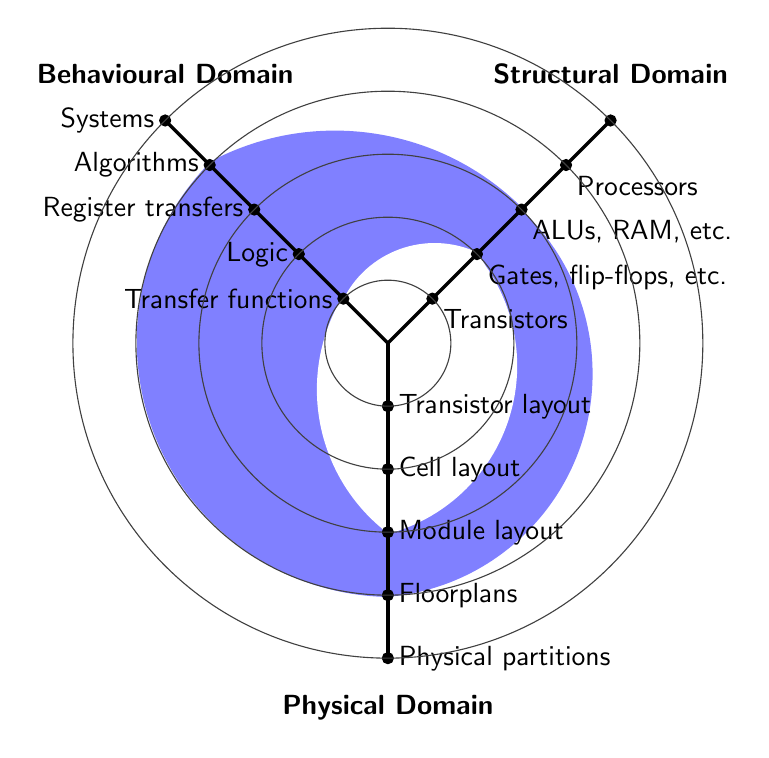
\begin{tikzpicture}[>=stealth,join=bevel,font=\sffamily,auto]
    \coordinate (behaviouralNode) at (135:4cm);
    \coordinate (structuralNode) at (45:4cm);
    \coordinate (physicalNode) at (270:4cm);
    \coordinate (originNode) at (0:0cm);

\draw[very thick,blue!50,fill=blue!50] (barycentric cs:physicalNode=0.8,originNode=0.2) arc (-85:50:2.825) -- (barycentric cs:structuralNode=0.6,originNode=0.4) arc (45:117.5:3.3525) -- (barycentric cs:behaviouralNode=0.8,originNode=0.2) arc (136:267.5:3.225) -- cycle; 
\draw[very thick,white,fill=white] (barycentric cs:physicalNode=0.6,originNode=0.4) arc (-75:35:2.1875) -- (barycentric cs:structuralNode=0.4,originNode=0.6) arc (65:250:1.275) -- (barycentric cs:behaviouralNode=0.2,originNode=0.8) arc (149.5:230:2.275) -- cycle; 

%\draw[very thick,blue!25,fill=blue!50] (barycentric cs:physicalNode=0.8,originNode=0.2) -- (barycentric cs:structuralNode=0.6,originNode=0.4) -- (barycentric cs:behaviouralNode=0.8,originNode=0.2) -- cycle;
%\draw[very thick,blue!25,fill=white] (barycentric cs:physicalNode=0.6,originNode=0.4) -- (barycentric cs:structuralNode=0.4,originNode=0.6) -- (barycentric cs:behaviouralNode=0.4,originNode=0.6) -- cycle;

    \node [above=1em] at (behaviouralNode) {\textbf{Behavioural Domain}};
    \node [above=1em] at (structuralNode) {\textbf{Structural Domain}};
    \node [below=1em] at (physicalNode) {\textbf{Physical Domain}};

    \draw[-, very thick] (behaviouralNode.south) -- (0,0) node[left,pos=0]{Systems} node[left,pos=0.2]{Algorithms} node[left,pos=0.4]{Register transfers} node[left,pos=0.6]{Logic} node[left,pos=0.8]{Transfer functions};

    \draw[-, very thick] (structuralNode.south) -- (0,0) node[pos=0]{ } node[pos=0.2]{Processors} node[pos=0.4]{ALUs, RAM, etc.} node[pos=0.6]{Gates, flip-flops, etc.} node[pos=0.8]{Transistors};

    \draw[-, very thick] (physicalNode.south) -- (0,0) node[right,pos=0]{Physical partitions} node[right,pos=0.2]{Floorplans} node[right,pos=0.4]{Module layout} node[right,pos=0.6]{Cell layout} node[right,pos=0.8]{Transistor layout};

    \draw[fill] (barycentric cs:behaviouralNode=1.0,originNode=0) circle (2pt);
    \draw[fill] (barycentric cs:behaviouralNode=0.8,originNode=0.2) circle (2pt);
    \draw[fill] (barycentric cs:behaviouralNode=0.6,originNode=0.4) circle (2pt);
    \draw[fill] (barycentric cs:behaviouralNode=0.4,originNode=0.6) circle (2pt);
    \draw[fill] (barycentric cs:behaviouralNode=0.2,originNode=0.8) circle (2pt);

    \draw[fill] (barycentric cs:structuralNode=1.0,originNode=0) circle (2pt);
    \draw[fill] (barycentric cs:structuralNode=0.8,originNode=0.2) circle (2pt);
    \draw[fill] (barycentric cs:structuralNode=0.6,originNode=0.4) circle (2pt);
    \draw[fill] (barycentric cs:structuralNode=0.4,originNode=0.6) circle (2pt);
    \draw[fill] (barycentric cs:structuralNode=0.2,originNode=0.8) circle (2pt);

    \draw[fill] (barycentric cs:physicalNode=1.0,originNode=0) circle (2pt);
    \draw[fill] (barycentric cs:physicalNode=0.8,originNode=0.2) circle (2pt);
    \draw[fill] (barycentric cs:physicalNode=0.6,originNode=0.4) circle (2pt);
    \draw[fill] (barycentric cs:physicalNode=0.4,originNode=0.6) circle (2pt);
    \draw[fill] (barycentric cs:physicalNode=0.2,originNode=0.8) circle (2pt);

    \draw[black!75] (0,0) circle (4.0cm);
    \draw[black!75] (0,0) circle (3.2cm);
    \draw[black!75] (0,0) circle (2.4cm);
    \draw[black!75] (0,0) circle (1.6cm);
    \draw[black!75] (0,0) circle (0.8cm);

  \end{tikzpicture}
\caption{Gajski-Kuhn Y-grafikoan proiektuaren abstrakzio maila.} 
\label{fig:ychart}
\end{figure}
%Anie - ohkis.sourceforge.net
%Unai Martinez Corral
%umartinez012@ikasle.ehu.es
%
% <- anie.tex

\section{Lizentziak eta aitorpenak}

Txantiloi hau hurrengo lizentziaren arabera eskaintzen da:

\begin{center}
\large\bfseries
Creative Commons Attribution-ShareAlike 3.0\\(CC BY-SA 3.0)
\end{center}

\begin{itemize}
\item{Egin ditzakezunak:
 \begin{description}
  \item[Banatzea]{Kopiatu, banatu eta hedatzea}
  \item[Moldatzea]{Lana egokitzea eta eratorriak egitea}
  \item[lana merkataritza helburuekin erabiltzea]{}
 \end{description}
}
\item{Hurrengoak bete bitartean:
 \begin{description}
  \item[Aitortzea]{Lanaren iturria aitortu behar da, \emph{Unai Martinez Corral} eta \emph{ITSAS}i erreferentzia eginez, eta \url{itsas.ehu.es/workgroups/latex} orrialdea aipatuz (baina lan eratorriek edo lanaren erabilerek hauen babesa dutela adierazi barik).}
  \item[Berdin partekatzea]{Lan hau moldatu edo egokituz gero, edo lan eratorririk sortzekotan, egindakoa banatzeko honetan erabilitako lizentzia berdina erabili behar da.}
 \end{description}
}
\end{itemize}

\begin{center}
\large\url{creativecommons.org/licenses/by-sa/3.0/es/legalcode.eu}
\end{center}

\bigskip
\bigskip

Aipatutako ITSASen lan taldeetako baliabideez gain, jarraian zerrendatutakoak erabili dira:

\begin{itemize}
\item{\textbf{TeXmaker} (\url{xm1math.net/texmaker}) \emph{Pascal Brachet}}
\item{\textbf{BibTeX} (\url{bibtex.org}) \emph{Oren Patashnik, Leslie Lamport, Oren Patashnik}}
\item{\LaTeX{} paketeak (\url{ctan.org/pkg/}):
 \begin{description}
 \item[import]{\emph{Donald Arseneau}}
 \item[inputenc]{\emph{Alan Jeffrey, Frank Mittelbach}}
 \item[babel]{\emph{Javier Bezos, Johannes L. Braams}}
 \item[geometry]{\emph{Hideo Umeki}}
 \item[graphicx]{\emph{David Carlisle}}
 \item[natbib]{\emph{Patrick W. Daly, Arthur Ogawa}}
 \item[caption]{\emph{Axel Sommerfeldt}}
 \item[indentfirst]{\emph{Davis Carlisle}}
 \item[multirow]{\emph{Piet van Oostrum, Jerry Leichter}}
 \item[amsmath]{\emph{The American Mathematical Society}}
 \item[eurofont]{\emph{Rowland McDonnell}}
 \item[xcolor]{\emph{Uwe Kern}}
 \item[listings]{\emph{Brooks Moses, Carsten Heinz}}
 \item[tikz,pgfplots]{\emph{Till Tantau, Christian Feuers{\"{a}}nger}}
 \item[tikz-timing]{\emph{Martin Scharrer}}
 \item[url]{\emph{Donald Arseneau}}
 \item[hyperref]{\emph{Heiko Oberdiek, Sebastian Rahtz}}
 \item[etoolbox]{\emph{Philipp Lehman}}
 \item[minitoc]{\emph{Jean-Pierre Drucbert}}
 \item[eso-pic]{\emph{Rolf Niepraschk}}
 \item[fancyhdr]{\emph{Piet van Oostrum}}
 \end{description}
}
\item{\textbf{QtikZ} (\url{hackenberger.at/blog/ktikz-editor-for-the-tikz-language}) \emph{Florian Hackenberger}}
\item{TikZ irudiak (\url{texample.net/tikz/examples/}):
 \begin{description}
  \item[Gajski-Kuhn Y-chart]{\emph{Ivan Griffin}} 
  \item[Control system principles]{\emph{Kjell Magne Fauske}}
  \item[Timing diagram with the tikz-timing package]{\emph{Martin Scharrer}}
 \end{description}
}
\end{itemize}

%\begin{center}
% 
\includegraphics[width=200pt]{./images/ccby.png}
%\end{center}
%
%Dokumentu hauek guztiak, iturri kodea izan ezik, Creative Commons By 3.0 (CC-by-3.0) lizentiak babesten ditu. Kopia, banaketa eta jendaurrean aurkeztea baimenduta daude, baita aldatzea eta moldatzea ere, betiere Unai Martinez Corral aipatuz autoretza aitortzen bada (baina ez honen, autorearen, babesa duela edo bere lanaren erabilera babesten duela aditzera emanez).
%
%\href{http://creativecommons.org/licenses/by/3.0/legalcode}{Lege testu} osoa \href{http://creativecommons.org}{Creative Commons} erakundearen web gunean dago eskuragarri::
%\begin{center}http://creativecommons.org/licenses/by/3.0/legalcode\end{center}
%
%\vspace{1cm}
%
%\begin{center}
% \includegraphics[width=100pt]{./images/gpl.png}
%\end{center}
%
%Programaren iturri kodea (bai mikrokontroladorerako C lengoiaian idatzitakoa, bai LabVIEW-rako era grafikoan egindakoa) GPL lizentziak babesten du, fitxategien goiburuek adierazten duten bezala. \ref{gpl} eranskinean lege testu osoa dago eskuragarri. \href{http://www.gnu.org}{GNU Proiektua}-ren web gunean ere aurkitu daiteke.\label{lic}
%Anie - ohkis.sourceforge.net
%Unai Martinez Corral
%umartinez012@ikasle.ehu.es
%
% <- anie.tex

\section{Teknikaren egoera eta ebatzien azterketa}
\end{verbatim}

Memoriaren atalak dituzten fitxategiak zuzenean \emph{include} edo \emph{input} bitartez kargatzen dira. Lehenengoa \emph{main.tex} fitxategian baino ezin daiteke erabili, beste fitxategi guztietan \emph{input} erabiltzen da.

\begin{verbatim}
\subincludefrom{./secta/}{secta_main}
\subincludefrom{./sectb/}{sectb_main}
\end{verbatim}

Hainbat fitxategi dituzten atalak karpeta banatuetan gordetzen dira eta \emph{main.tex}en fitxategi bakarra kargatzen da. Honek atal aldaketa txikiak eginez horiek banatu eta bakarrik konpilatzea ahalbidetzen du, eta egitura aldatu barik hainbat atal gehitzea.

\begin{verbatim}
\chapter{Neurketak eta kalkuluak} \DOmtls{\DOmtoc}
\subincludefrom{./measures/}{measures_main}

\chapter{Eranskinak} \DOmtls{\DOmtoc}
\attref
\subincludefrom{./att/}{att_main}
\ordref

\chapter{Baldintzen agiria} \DOmtls{\DOmtoc}
\subincludefrom{./cond/}{cond_main}

\chapter{Aurrekontua}
\end{verbatim}

Azaldutako tresna berdinak erabilita kargatzen dira hurrengo kapituluak. Ikus daitekeenez hauetan gaien aurkibidea aurkezten da soilik. \emph{Eranskinak} dokumentuaren edukia kargatu baino lehen adierazitako \emph{attref} komandoak atalen zenbakitzea alfabetora aldatzen du (ikus \emph{config\_index.tex}). Dokumentuaren bukaeran berriz ere bueltatzen da hasierako aurreko konfiguraziora (\emph{ordref}, ikus \emph{config\_basque.tex}).

\begin{verbatim}
\nocite{*}
\chapter{Bibliografia}
\bibliographystyle{ieeetr}
\fancyhead[L]{\slshape \nouppercase{\bibname}}
\bibliography{bibliography}
\end{verbatim}

Erreferentzia guztiak (estekatutakoak eta estekatu gabekoak) aurkezteko \emph{nocite{*}} deitu ostean, \emph{Bibliografia} kapitulua hasi, estiloa aukeratu, orrialde bat baino gehiago izatekotan itxura egokia aurkezteko goiburua moldatu eta \emph{bibligraphy.bib} fitxategia kargatzen du.

\begin{verbatim}
\end{document}
\end{verbatim}

\subsection*{config/config.tex}\addcontentsline{toc}{subsection}{config/config.tex}

\begin{verbatim}
\usepackage[utf8]{inputenc}
\end{verbatim}

Karaktereen kodeketa adierazteko.

\begin{verbatim}
\usepackage[spanish,basque]{babel} 
\selectlanguage{basque}
\end{verbatim}

Tituluak batez ere, eta beste hainbat aukera, lokalizatzeko. Gaztelera kargatzen da izen propioak erabiltzean \emph{ñ} eta azentu-markekin arazorik ez izateko. 

\begin{verbatim}
\usepackage[left=3.5cm, right=1.5cm, top=2.5cm, bottom=2.5cm]{geometry}
\end{verbatim}

Normak adierazitako marjinak ezartzeko.

\begin{verbatim}
\usepackage{graphicx}
\end{verbatim}

Irudiak txertatzeko.

\begin{verbatim}
\usepackage[numbers]{natbib}
\end{verbatim}

Erreferentzia bibliografikoak testuan adieraztean \emph{[X]} itxuraz adierazi daitezen.

\begin{verbatim}
\usepackage[font=scriptsize,format=plain,labelfont=bf,textfont=it,
            justification=centerlast]{caption}
\end{verbatim}

Irudi eta taulen oinen itxura moldatzeko.

\begin{verbatim}
\usepackage{indentfirst}
\end{verbatim}

\emph{babel} paketeak gazteleraz paragrafo bakoitzaren lehenengo lerroari ezkerreko marjina handiagoa jartzen dio, baina euskaraz ez. Honek egitera bortxatzen du, baina kontuz ibili beharko dugu irudiak eta taulak erdiratzerakoan.

\begin{verbatim}
\usepackage{multirow}
\end{verbatim}

Tauletan zutabe edo lerro anitz hartzen dituzten gelaxkak erabiltzeko.

\begin{verbatim}
\usepackage{eurofont}
\end{verbatim}

\euro{} sinboloa erabiltzeko.

\begin{verbatim}
\usepackage[usenames,dvipsnames]{xcolor}
\colorlet{urlcolor}{purple!65!black}
\colorlet{ilcolor}{violet!65!black}
\end{verbatim}

Esteketan, irudietan eta grafikoetan koloreak definitzeko aukera ugari izateko.

\begin{verbatim}
\usepackage{listings}
\lstset{
language=VHDL,
basicstyle=\color{Blue}\footnotesize\ttfamily,
commentstyle=\color{CadetBlue},
stringstyle=,
identifierstyle=\color{Black},
backgroundcolor=\color{black!10!white},
columns=fixed,
extendedchars=true,
breaklines=true,
numbers=none
}
\end{verbatim}

Lengoaia ezberdinetan idatzitako kodea dokumentuan txertatzeko. Eredu gisa erabili den VHDL kodea aurkezteko ausazko aurkezpenaren hautaketa.

\begin{verbatim}
\usepackage{tikz,pgfplots}
\usetikzlibrary{shapes,arrows}
\usepackage{tikz-timing}
\end{verbatim}

Irudiak, grafikoak eta kronogramak egiteko.

\begin{verbatim}
\usepackage[hyphens]{url}
\usepackage[
 bookmarks=true,
 unicode=true,
 pdftitle={Karrera Amaierako Proiektuak idazteko LaTeX txantiloia},
 pdfsubject={},
 pdfauthor={Unai Martinez Corral},
 linktoc=all,
 colorlinks=true,
 linkcolor=ilcolor,
 urlcolor=urlcolor,
 citecolor=Blue,
 plainpages=false,
]{hyperref}
\end{verbatim}

Dokumentuko erreferentziak estekatzeko eta irteerako PDF fitxategiaren propietateak ezartzeko.

\begin{verbatim}
\parskip=2mm
\end{verbatim}

Paragrafoen arteko tartea ezartzea.

\begin{verbatim}
\usepackage{amsmath}
\numberwithin{figure}{chapter}
\numberwithin{table}{chapter}
\numberwithin{equation}{chapter}
\end{verbatim}

Irudi, taula eta ekuazioen zenbakitzea kapitulu bakoitzean berrabiatzeko.

\begin{verbatim}
\usepackage{etoolbox}
\end{verbatim}

Komandoei dei egitean exekutatu baino lehen bitarteko ekintzak burutzeko.

\begin{verbatim}
% Karrera Amarierako Proiektua egiteko LaTeX txantiloia
% itsas.ehu.es/workgroups/latex
% Unai Martinez Corral
% umartinez012@ikasle.ehu.es
%
% <- config.tex

\newcommand\subsectiontitle{}
\newcommand{\titlesubsection}[1]{\subsection{#1}\renewcommand{\subsectiontitle}{#1}\ttlsbs}

\newcommand\sectiontitle{}
\newcommand\hdrgb{\ifhmode\par\fi\removelastskip\vskip 5ex\goodbreak}
\newcommand\hdrpre{\noindent\leavevmode\vskip -3em}
\newcommand\hdrdec{\vskip -2ex\noindent\hrulefill\vskip -3.75ex\nobreak\noindent\hrulefill}%\vskip 1.5em}
\newcommand\hdrpost{\nobreak\vskip 2ex\nobreak}
\makeatletter
\def\section{\@ifstar\unnmbsect\nmbsect}
\def\nmbsect{\@ifnextchar[%]
 \nmbsectwithtwoarguments\nmbsectwonearg}
\def\unnmbsect{\@ifnextchar[%]
 \unnmbsectwithtwoarguments\unnmbsectwonearg}
\def\nmbsectwonearg#1{\nmbsectwithtwoarguments[#1]{#1}}
\def\unnmbsectwonearg#1{\unnmbsectwithtwoarguments[#1]{#1}}
\def\nmbsectwithtwoarguments[#1]#2{%  
 \hdrgb \refstepcounter{section} \hbox to \hsize{\vbox{%
  \hdrpre{\Huge\bfseries\raggedleft \thesection\ \\ \LARGE #2\par}\hdrdec}} \hdrpost
 \addcontentsline{toc}{section}{\protect\numberline{\thesection} #1}
 \renewcommand\sectiontitle{#2}}
\def\unnmbsectwithtwoarguments[#1]#2{%
 \hdrgb \hbox to \hsize{\vbox{%
  \hdrpre{\LARGE\bfseries\raggedleft #2\par}\hdrdec}} \hdrpost
 \renewcommand\sectiontitle{#2}}
\makeatother

\newcommand\chaptertitle{}
\makeatletter
\def\@makeschapterhead#1{\section*{#1}}
\def\@makechapterhead#1{%
\setcounter{page}{0}
\thispagestyle{empty}
\AddToShipoutPicture*{\chapterback}
\vspace*{1em}
\begin{minipage}{\textwidth}%Anie - ohkis.sourceforge.net
%Unai Martinez Corral
%umartinez012@ikasle.ehu.es
%
% <- anie_config...

\begin{minipage}{.1125\textwidth}
\centering
\includegraphics[width=.95\textwidth]{./images/ehu.png}
\end{minipage}
\begin{minipage}{.7\textwidth}
\begin{center}
{\bfseries BILBOKO INDUSTRIA INGENIARITZA TEKNIKOKO\\UNIBERTSITATE ESKOLA}

\vspace{5pt}
\scriptsize INDUSTRIA INGENIARITZA TEKNIKOA: INDUSTRIA ELEKTRONIKA

\vspace{5pt}
KARRERA AMAIERAKO PROIEKTUA
\end{center}
\end{minipage}
\begin{minipage}{.1125\textwidth}
\centering
\includegraphics[width=.95\textwidth]{./images/euiti.png}
\end{minipage}
\end{minipage}

\vspace*{180\p@}%
{\parindent \z@ \raggedright \normalfont
\ifnum \c@secnumdepth >\m@ne
\Huge\bfseries\centering\thechapter.\space\@chapapp:\par\nobreak
\fi
\interlinepenalty\@M
\Huge\bfseries #1\par\nobreak
}
\renewcommand\chaptertitle{#1}
\vspace*{200pt}
\begin{minipage}{\textwidth}%Anie - ohkis.sourceforge.net
%Unai Martinez Corral
%umartinez012@ikasle.ehu.es
%
% <- anie_config...

\begin{tabular}[c]{| p{0.4375\textwidth} | p{0.4375\textwidth} |}
\hline
&\\
\hspace{5pt}\textbf{IKASLEAREN DATUAK}&\hspace{5pt}\textbf{ZUZENDARIAREN DATUAK}\\
&\\
\begin{minipage}{.4375\textwidth}\centering\large Izena 1.Abizena 2.Abizena\\\normalsize\ttfamily i1abizenaxxx@ikasle.ehu.es\\00000000-X\end{minipage}
&
\begin{minipage}{.4375\textwidth}\centering\large Izena 1.Abizena 2.Abizena\\\normalsize\ttfamily izena.abizena1@ehu.es\\Sailaren Izena\end{minipage}\\
&\\
&\\
&\\
&\\
\hspace{10pt}SIN.:&\hspace{10pt}SIN.:\\
\hspace{10pt}DATA: \gaur&\hspace{10pt}DATA:\\
&\\
\hline
\end{tabular}\end{minipage}
\clearpage
}
\makeatother
% Karrera Amarierako Proiektua egiteko LaTeX txantiloia
% itsas.ehu.es/workgroups/latex
% Unai Martinez Corral
% umartinez012@ikasle.ehu.es
%
% <- config.tex

\usepackage{eso-pic}
\newcommand\chapterback{%
\normalcolor\linethickness{1pt}%
\AtTextLowerLeft{ \put(-\LenToUnit{\parindent},0){%
 \framebox(\LenToUnit{\textwidth},\LenToUnit{\textheight}){} }%
}}

\usepackage{fancyhdr}
\pagestyle{empty}

\newcommand\myfoot{
\fancyfoot[L]{\slshape \chaptertitle}  \fancyfoot[C]{\thepage}  \fancyfoot[R]{ITSAS - UPV/EHU}
}

\fancypagestyle{firstbody}{ \fancyhf{}
\renewcommand{\headrulewidth}{0pt}
\renewcommand{\footrulewidth}{0.4pt}
\myfoot}

\fancypagestyle{body}{ \fancyhf{}
\renewcommand{\headrulewidth}{0.4pt}
\renewcommand{\footrulewidth}{0.4pt}
\fancyhead[L]{\slshape \nouppercase{\thesection~\sectiontitle}}
\myfoot}

\renewcommand{\headrulewidth}{0pt}
\renewcommand{\footrulewidth}{0pt}
\renewcommand{\footnoterule}{\vspace*{0pt}
  \noindent\rule{1cm}{0.4pt}\vspace*{5pt}}
  
\makeatletter
\pretocmd{\section}{\thispagestyle{firstbody}}{}{}

\newcommand\subsectionhdr{\slshape \nouppercase{\thesubsection~\subsectiontitle}}
\pretocmd{\subsection}{\fancyhead[R]{}}{}{}
\newcommand\ttlsbs{\fancyhead[R]{\subsectionhdr}}{}{}
% Karrera Amarierako Proiektua egiteko LaTeX txantiloia
% itsas.ehu.es/workgroups/latex
% Unai Martinez Corral
% umartinez012@ikasle.ehu.es
%
% <- config.tex

\addto\captionsbasque{\renewcommand{\chaptername}{Dokumentua}}

\makeatletter 
\renewcommand{\fnum@figure}{\thefigure~\figurename}
\renewcommand{\fnum@table}{\thetable~\tablename}

\newcommand{\ordref}{
\renewcommand*\thesection{\arabic{section}.}
\renewcommand*\thesubsection{\arabic{section}.\arabic{subsection}.}
\renewcommand*\thesubsubsection{\arabic{section}.\arabic{subsection}.\arabic{subsubsection}.}

\renewcommand\thefigure{\arabic{chapter}.\arabic{figure}.}
\renewcommand\thetable{\arabic{chapter}.\arabic{table}.}
\renewcommand\theequation{\arabic{chapter}.\arabic{equation}}
}
\makeatother

\newcommand\gaur{{\number\year}ko\space\ifcase\month\or
 urtarrila\or otsaila\or martxoa\or apirila\or maiatza\or ekaina\or uztaila\or
 abuztua\or iraila\or urria\or azaroa\or abendua\fi ren~\number\day a}
% Karrera Amarierako Proiektua egiteko LaTeX txantiloia
% itsas.ehu.es/workgroups/latex
% Unai Martinez Corral
% umartinez012@ikasle.ehu.es
%
% <- config.tex

\makeatletter
\newcommand\attref{}
\pretocmd{\attref}{
\renewcommand*\thesection{\Alph{section}.}
\renewcommand\thefigure{\Alph{section}.\arabic{figure}.}
\renewcommand\thetable{\Alph{section}.\arabic{table}.}
\renewcommand\theequation{\Alph{section}.\arabic{equation}}
\fancyhead[R]{}
}{}{}
\makeatother

\makeatletter
\newcommand*{\ititle}{}
\newcommand*{\DOititle}{}
\newcommand*{\DOmnow}{}

\newcommand*\DOtls{\DOmpre\DOtocloflot\DOmpost}
\newcommand*\DOmtls[1]{\DOmcpre\DOmtitle #1 \DOmcpost}

\newcommand*\DOmpre{\renewcommand{\thepage}{\roman{page}}}
\newcommand*\DOmcpre{\clearpage\setcounter{page}{1}
\renewcommand*{\thepage}{\arabic{chapter}-\roman{page}}}
\newcommand*\DOmpost{ \renewcommand{\thepage}{\arabic{chapter}-\arabic{page}}
\pagestyle{body} }
\newcommand*\DOmcpost{\setcounter{page}{1}\DOmpost}

\newcommand*\DOtocloflot{
\renewcommand*{\ititle}{\contentsname} \renewcommand*{\DOititle}{\tableofcontents}
\renewcommand*{\DOmnow}{} \DOmhere
\renewcommand*{\ititle}{\listfigurename} \renewcommand*{\DOititle}{\listoffigures}
\renewcommand*{\DOmnow}{} \DOmhere
\renewcommand*{\ititle}{\listtablename} \renewcommand*{\DOititle}{\listoftables}
\renewcommand*{\DOmnow}{} \DOmhere
}

\newcommand*\DOmhere{
\fancyhead[L]{\slshape \nouppercase{\ititle}}
\DOititle \addcontentsline{toc}{section}{\ititle}
\DOmnow \clearpage}

\newcommand*\DOmtitle{\renewcommand*{\DOititle}{\section*{\ititle}}}

\newcommand*\DOmtoc{ \renewcommand*{\ititle}{\contentsname} \renewcommand*{\DOmnow}{\minitoc}
\DOmhere}
\newcommand*\DOmlof{ \renewcommand*{\ititle}{\listfigurename} \renewcommand*{\DOmnow}{\minilof}
\DOmhere}
\newcommand*\DOmlot{ \renewcommand*{\ititle}{\listtablename} \renewcommand*{\DOmnow}{\minilot}
\DOmhere}
\newcommand*\DOmlos{ \renewcommand*{\ititle}{Ikurren Zerrenda} \renewcommand*{\DOmnow}{%Anie - ohkis.sourceforge.net
%Unai Martinez Corral
%umartinez012@ikasle.ehu.es
%
% <- anie.tex

\subsection*{Letra larriak}

\begin{tabular}{c c l}
$Y$ & --- & .\\
$E$ & --- & .\\
$U$ & --- & .\\
$T_s$ & --- & .\\
\end{tabular}

\subsection*{Letra xeheak}
\begin{tabular}{c c l}
$y$ & --- & .\\
$e$ & --- & .\\
$u$ & --- & .\\
$z^{-1}$ & --- & .\\
\end{tabular}

\subsection*{Letra grekoak}
\begin{tabular}{c c l}
$\omega$ & --- & Abiadura angeluarra.\\
\end{tabular}}
\DOmhere}
\makeatother

\makeatletter
\renewcommand\paragraph{\@startsection{paragraph}{4}{\z@}
  {3.25ex \@plus 1ex \@minus .2ex}{.01pt}%
  {\normalfont\normalsize\bfseries}%
}
\makeatother

\makeatletter
\renewcommand*\l@section{\@dottedtocline{1}{1.5em}{1em}}
\renewcommand*\l@subsection{\@dottedtocline{2}{3.35em}{2em}}
\renewcommand*\l@subsubsection{\@dottedtocline{3}{5.4em}{3em}}
\renewcommand*\l@paragraph{\@dottedtocline{4}{9.4em}{4em}}
\makeatother
\end{verbatim}

Funtzio zehatzen konfigurazioa: portadak eta atalek goiburuak, bestelako goiburu eta oinak, euskaraz erabiltzeko hobekuntzak eta aurkibideak aurkeztea.

\begin{verbatim}
\usepackage[basque,loose]{minitoc}
%\usepackage{mtcoff}
\setcounter{minitocdepth}{4}
\setlength{\mtcindent}{0pt}
\renewcommand{\mtcfont}{\small\rm}
\renewcommand{\mtcSfont}{\small\bf} 
\nomtcrule \nomlfrule \nomltrule
\end{verbatim}

Kapitulu bakoitzean aurkibideak eta zerrendak aurkeztea ahalbidetzen duen paketea kargatzea eta hainbat parametro ezartzea. Hauen artean garrantzitsuena \emph{setcounter{minitocdepth}} dugu, aurkibideek aurkeztuko duten sakontasuna adierazten baitu: 0-kapitulua, 1-atala, 2-azpiatala, 3-azpiazpiatala edo 4-paragrafoa. Besteek letra mota ezartzen dute eta zerrenden inguruko lerroak ezabatzen dituzte.

\begin{verbatim}
\newcommand{\DOpresetDOtitlepg}{
\ordref
\setcounter{secnumdepth}{3}
\setcounter{tocdepth}{1}
\addtocounter{chapter}{-1}
\dominitoc[e]
\dominilof[e]
\dominilot[e]
%Anie - ohkis.sourceforge.net
%Unai Martinez Corral
%umartinez012@ikasle.ehu.es
%
% <- anie.tex

\AddToShipoutPicture*{\chapterback}
\begin{titlepage}
\thispagestyle{empty}
\vspace*{1em}
\begin{minipage}{\textwidth}%Anie - ohkis.sourceforge.net
%Unai Martinez Corral
%umartinez012@ikasle.ehu.es
%
% <- anie_config...

\begin{minipage}{.1125\textwidth}
\centering
\includegraphics[width=.95\textwidth]{./images/ehu.png}
\end{minipage}
\begin{minipage}{.7\textwidth}
\begin{center}
{\bfseries BILBOKO INDUSTRIA INGENIARITZA TEKNIKOKO\\UNIBERTSITATE ESKOLA}

\vspace{5pt}
\scriptsize INDUSTRIA INGENIARITZA TEKNIKOA: INDUSTRIA ELEKTRONIKA

\vspace{5pt}
KARRERA AMAIERAKO PROIEKTUA
\end{center}
\end{minipage}
\begin{minipage}{.1125\textwidth}
\centering
\includegraphics[width=.95\textwidth]{./images/euiti.png}
\end{minipage}
\end{minipage}

\begin{center}
\vspace*{25pt}

\begin{minipage}{.8\textwidth}
\centering
\LARGE
{\bfseries Karrera Amaierako Proiektuak idazteko\\\LaTeX{} txantiloia}

\vspace*{25pt}

\includegraphics[width=200pt]{./images/logo.png}
\end{minipage}

\vspace{25pt}
\hspace{3em}
\begin{minipage}{.425\textwidth}
\LARGE
0. Aurkibide orokorra\\
1. Memoria\\
2. Neurketak eta kalkuluak\\
3. Eranskinak\\
4. Baldintzen agiria\\
5. Aurrekontua\\
6. Bibliografia\\
\end{minipage}
\end{center}

\begin{minipage}{\textwidth}%Anie - ohkis.sourceforge.net
%Unai Martinez Corral
%umartinez012@ikasle.ehu.es
%
% <- anie_config...

\begin{tabular}[c]{| p{0.4375\textwidth} | p{0.4375\textwidth} |}
\hline
&\\
\hspace{5pt}\textbf{IKASLEAREN DATUAK}&\hspace{5pt}\textbf{ZUZENDARIAREN DATUAK}\\
&\\
\begin{minipage}{.4375\textwidth}\centering\large Izena 1.Abizena 2.Abizena\\\normalsize\ttfamily i1abizenaxxx@ikasle.ehu.es\\00000000-X\end{minipage}
&
\begin{minipage}{.4375\textwidth}\centering\large Izena 1.Abizena 2.Abizena\\\normalsize\ttfamily izena.abizena1@ehu.es\\Sailaren Izena\end{minipage}\\
&\\
&\\
&\\
&\\
\hspace{10pt}SIN.:&\hspace{10pt}SIN.:\\
\hspace{10pt}DATA: \gaur&\hspace{10pt}DATA:\\
&\\
\hline
\end{tabular}\end{minipage}
\end{titlepage}
\clearpage

\clearpage\pagestyle{body}
}
\end{verbatim}

Dokumentua hasi eta berehala \emph{config\_basque.tex} fitxategian definitutako \emph{ordref} komandoak euskaraz elementuen izenak ondo adierazi daitezen moldaketak burutzen ditu.

Atalak zenbakitzeko erabiliko den sakontasuna adierazten da ondoren (3-azpiazpiatala), eta aurkibide nagusiak aurkeztuko duena (1-atala). Kapituluen zenbakitzea zeroan hasteko izendatuari bat kentzen zaio.

\emph{minitoc}ek eskatutako komandoak adierazten dira, izenbururik gabe aurkezteko parametroarekin (\emph{[e]}). \emph{config\_index.tex} fitxategian ikus daitekeenez izenburuak banaturik sortzen dira, lan osoaren estiloa mantentzeko.

Portada aurkezten da azkenik, eta berehala orrialde huts berri batean estilo orokorra ezarri.